\section{Présentation du sujet}
\paragraph{}
\vspace{-2em}
Au cours de mon stage chez Amazon, j'ai été impliqué dans un projet passionnant axé sur la redéfinition des régions(Region Definition Services). L'objectif principal de cette initiative était de remplacer les régions géographiques actuelles, définies par les pays, par des régions de vente mieux adaptées à la capacité opérationnelle d'Amazon. Ce projet revêt une importance stratégique, car il vise à aligner de manière plus efficace la structure régionale avec les exigences opérationnelles et la dynamique du marché. 
\paragraph{}
\vspace{-2em}
La mise en œuvre de ce projet vise à mieux accompagner le projet principal en fournissant un soutien essentiel à son développement. En redéfinissant les régions de vente, notre objectif est de créer un environnement plus propice au projet principal, lui permettant de s'adapter de manière plus flexible aux exigences du marché et aux défis opérationnels. 
\subsection{Connaissances préalables}
\paragraph{}
\vspace{-2em}
Avant de présenter le projet, il est nécessaire de présenter quelques connaissances préalables. 
\paragraph{}
\vspace{-2em}

\begin{itemize}
    \item \textbf{FC(Fulfillment Center)}: Un FC est un centre de distribution d'Amazon. Il s'agit d'un entrepôt où les produits sont stockés et expédiés aux clients.
    \item \textbf{SC(Sort Center)}: Un SC est un centre de tri d'Amazon. Il s'agit d'un centre où les colis sont triés et expédiés aux clients.
    \item \textbf{DS(Delivery Station)}: Un DS est une station de livraison d'Amazon. Il s'agit d'un centre à partir d'où les colis sont livrés aux clients.
    \item \textbf{Placement system}: Le placement system est un système qui permet de déterminer le FC dans lequel les stocks d'un produit doivent être placés. Il s'agit d'un système qui permet de déterminer le FC le plus adapté pour chaque produit.
\end{itemize}

\paragraph{}
\vspace{-2em}
Le voyage d'un produit peut être résumé comme suit:
\begin{itemize}
    \item \textbf{Achat et stockage}: Amazon achète des produits auprès des fournisseurs et les stocke dans les FC. Au cours de cette étape, le \textbf{Placement system} détermine le FC pour stocker les produits.
    \item \textbf{Commande et livraison}: Les clients passent des commandes sur le site web d'Amazon. Les produits sont expédiés aux clients à partir des FC.
\end{itemize}
\paragraph{}
\vspace{-2em}
Selon le passage entre ces centres, nous pouvons diviser le processus de livraison en trois parties:
\begin{itemize}
    \item \textbf{First mile}: Le premier kilomètre du processus de livraison. Il s'agit du passage entre le FC et le SC.
    \item \textbf{Middle mile}: Le kilomètre du milieu du processus de livraison. Il s'agit du passage entre le SC et le DS.
    \item \textbf{Last mile}: Le dernier kilomètre du processus de livraison. Il s'agit du passage entre le DS et le client.
\end{itemize}

Il faut tenir en compte que tous les trois passages vont engendrer des coûts. Par exemple, le passage entre le FC et le SC va engendrer des coûts de transport, et le passage entre le SC et le DS va engendrer des coûts de tri. Dans un cas spécific, le colis peut directement être expédié depuis le FC à le DS, sans passer par un SC. Nous l'appelons \textbf{DI}, acronyme de \textbf{Direct Injection}.

\subsection{Projet principal: Projet Möbius}
\paragraph{}
\vspace{-2em}
Le \textbf{Placement system} utilisent les coûts de transport réels et la vitesse historique à partir de la période des trois dernières semaines la plus récente. En tant que tels, les systèmes de placement ne sont pas conscients des éventuels changements dans la conception du réseau de transport. Par conséquent, le \textbf{Placement system} n'est pas en mesure de réagir rapidement aux changements de conception du réseau de transport. Il a tendance de placer les stocks d'un même produit dans le même FC, à la place de les placer dans des FC différents. 
\paragraph{}
\vspace{-2em}
En examinant les stations DIG1 et DRM2 dans la zone statistique métropolitaine de Londres (MSA), les deux sont directement connectées à LCY2 et LCY3 (Figure suivante) avec une heure limite de commande à minuit et des coûts d'expédition similaires. 
Le \textbf{Placement system} ne sépare pas les stock des deux type de produits dans les deux FC. 

\paragraph{}
\vspace{-2em}
Cette décision, entraînant une diminution des stocks partagés entre LCY2 et LCY3, nous oblige à maintenir des voies directes (DIs) à partir des deux centres de traitement (FCs) vers les deux sites de distribution (DS). Cependant, si nos systèmes recommandaient de diviser les colis et de les répartir pour augmenter la disponibilité à LCY2 et LCY3, il serait probablement possible de retirer deux DIs en passant le colis par un SC(Figure de droite).

\paragraph{}
\vspace{-2em}
Après la répartition, nous avons des stocks des deux produits dans tous les deux FC. Selon la distance, les coûts \texttt{b} et \texttt{c} deviendraient plus faibles. Alors que les coûts \texttt{a} et \texttt{d} deviendraient plus élevés. Les avantages liés aux coûts de transport longue distance compenseraient alors l'impact négatif sur les coûts et la vitesse de la chaîne logistique.

\begin{figure}[htbp]
    \centering
    \includegraphics[width=0.8\linewidth]{./Graphismes-UTC/logos/Amazon/mobius schema 1.pdf}\hfill
    %\vspace{-1em}
    \caption{Un exemple des stocks distribués}
\end{figure}

\subsection{Redéfinition des régions}
\subsubsection{Contexte}
\paragraph{}
\vspace{-2em}
Les régions géographiques existantes sont définies par chaque pays et l'Union Européenne. 
Cette nomenclature s'appelle \textbf{NUTS}(Nomenclature des unités territoriales statistiques). Il s'agit d'un découpage territorial destiné à faciliter les comparaisons entre pays, ou entre régions, d'un même ensemble.
\paragraph{}
\vspace{-2em}
Ces unités territoriales sont définies uniquement pour les besoins statistiques et ne constituent pas forcément des unités administratives officielles, mais souvent des groupements de ces unités administratives, en fonction de leur population résidente moyenne dans le pays correspondant.
\paragraph{}
\vspace{-2em}
Il existe trois niveaux de NUTS, qui sont définis comme suit:
\begin{itemize}
    \item NUTS 1: Les régions de niveau 1 sont les régions les plus grandes. Elles sont utilisées pour les comparaisons entre pays. Il y a 98 régions de niveau 1 en Europe.
    \item NUTS 2: Les régions de niveau 2 sont les régions intermédiaires. Elles sont utilisées pour les comparaisons entre régions. Il y a 276 régions de niveau 2 en Europe.
    \item NUTS 3: Les régions de niveau 3 sont les régions les plus petites. Elles sont utilisées pour les comparaisons entre régions. Il y a 1342 régions de niveau 3 en Europe.
\end{itemize}
\begin{figure}[H]
    \centering
    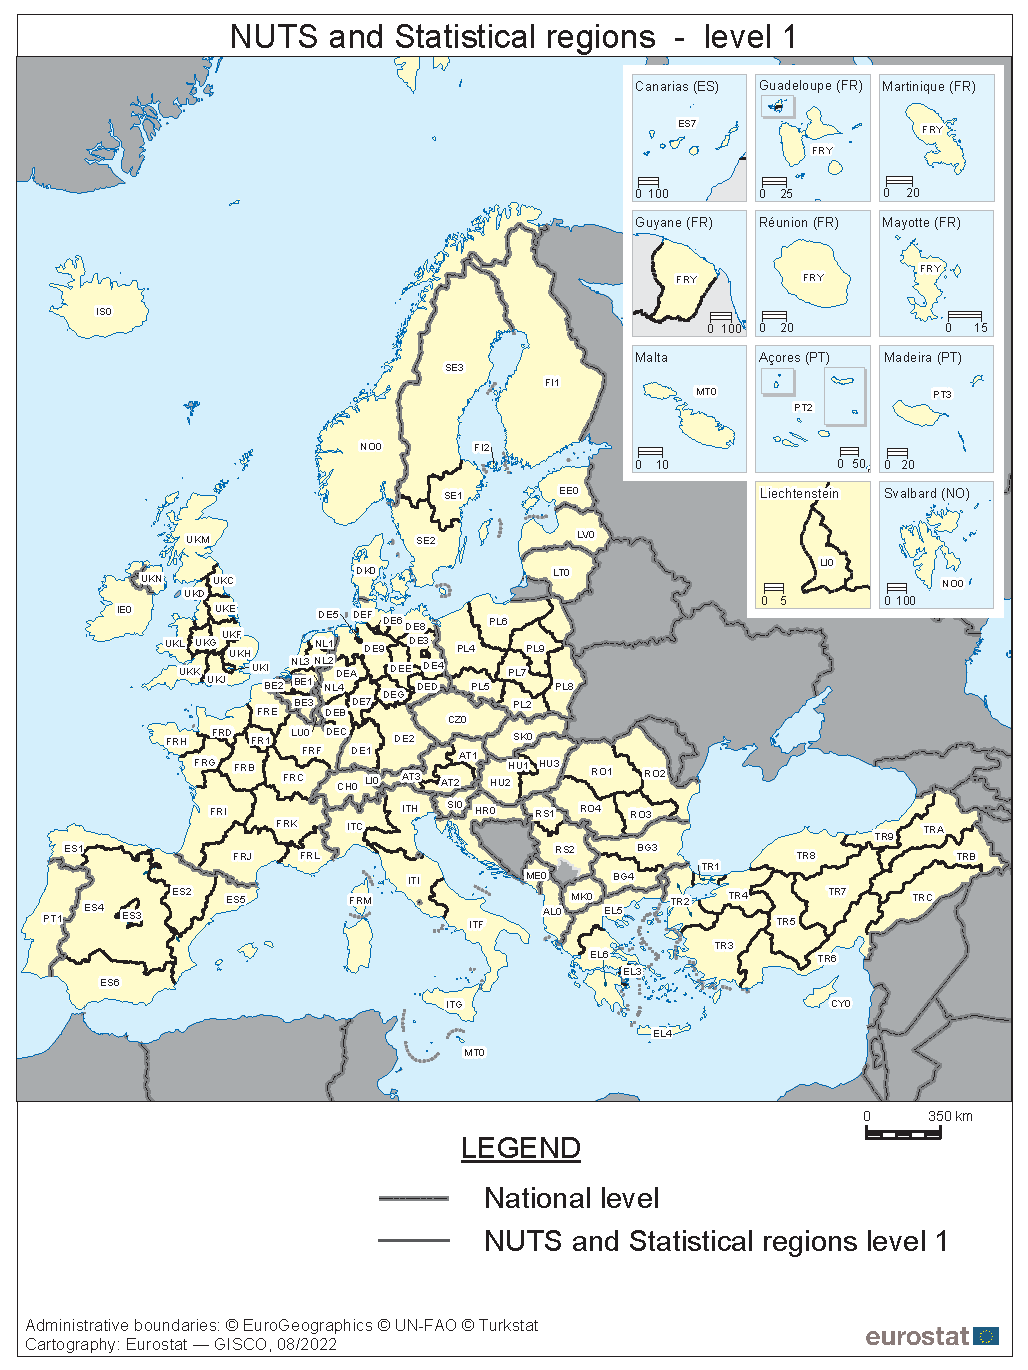
\includegraphics[width=0.45\linewidth]{./Graphismes-UTC/logos/Amazon/NUTS1.pdf}\hfill
    %\vspace{-1em}
    \caption{Plan de la NUTS1}
\end{figure}

Lors du déroulement de projet Möbius, il a été observé que les régions existantes ne sont pas adaptées aux exigences opérationnelles et à la dynamique du marché. En effet, les régions actuelles sont définies par les pays, ce qui ne permet pas de répondre aux besoins opérationnels. 

\paragraph{}
\vspace{-2em}
Nous pouvons relever les problèmes suivants:
\begin{itemize}
    \item Les régions eux-mêmes ne sont pas logiques. Par exemple, la région NUTS1 ES30 en Espagne est bordée par une autre région, et à première vue, il semble plus logique que ces deux régions soient fusionnées.
    \begin{figure}[htbp]
        \centering
        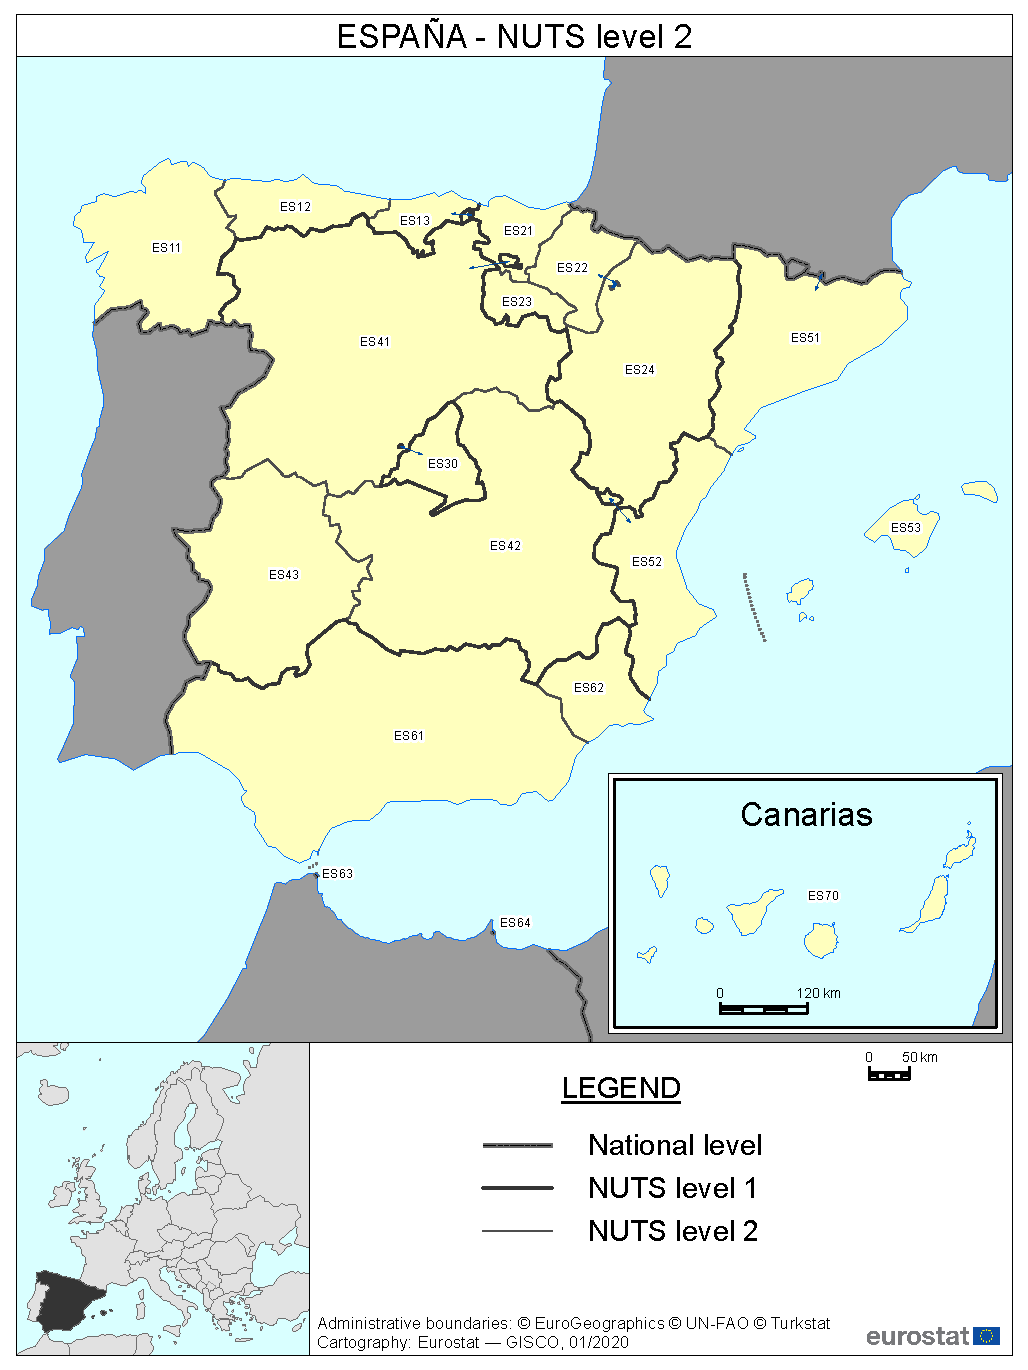
\includegraphics[width=0.6\linewidth]{./Graphismes-UTC/logos/Amazon/NUTS-2-ES.pdf}\hfill
        %\vspace{-1em}
        \caption{Plan de la NUTS1/2 en Espagne}
    \end{figure}
    \item Parmi les NUTS1, nous obervons des régions assez longues. Dans ce cas-là, il se pourrait que les communes aux extrémités d'une région soient plus proches d'un autre FC situé dans une autre région que de la leur. Par exemple, la région ES52 en Espagne est très longue, et les communes aux extrémités de cette région peut être couvert par un autre dans une autre région. Par contre, le système actuel ne permet pas de prendre en compte ce genre de situation. Ce dernier attribue encore ces communes au FC de ES52.
\end{itemize}
\paragraph{}
\vspace{-2em}
En plus, le \textbf{Placement system} agrègent les coûts de transport et la vitesse au niveau du code géographique NUTS1. En général, il y a généralement 10 codes NUTS1 dans chaque pays de l'Union européenne, tandis que la granularité pertinente pour le réseau de transport est le niveau de la station de livraison.
\paragraph{}
\vspace{-2em}
En ne considérant que la connectivité moyenne agrégée au niveau NUTS1, les systèmes ratent l'opportunité d'obtenir une exécution moins chère/plus rapide pour les sous-régions.
\subsubsection{Objectifs}
\paragraph{}
\vspace{-2em}
L'objectif, dans ce cas-là, comprend deux aspects principaux:
    \begin{itemize}
    \item Redéfinir les régions de vente pour mieux répondre aux exigences opérationnelles et à la dynamique du marché.
    \item Créer un environnement plus propice au projet principal, lui permettant de s'adapter de manière plus flexible aux exigences du marché et aux défis opérationnels.
    \end{itemize}
\paragraph{}
\vspace{-2em}
\subparagraph{Un sous-paragraphe}
Lorem ipsum dolor sit amet
\section*{Une section non numérotée}
\addcontentsline{toc}{section}{Une section non numérotée}